\section{Spannungsregler/Stromversorgung} 
	\subsection{Lineare Spannungsregler} 
		Für alle linearen Spannungsregler gilt: 
		\begin{equation*}
			P_{V}=(V_{E}-V_{a}) \cdot I_{a}
		\end{equation*}
		Einsatz für geringer Spannungsunterschied zwischen Eingangsspannung und der
		geregelten Ausgangsspannung \\
		
		\subsubsection{Qualitätsmasse}
			\begin{tabular}{l l}
				Relativer Stabilisierungsfaktor & $S' = \frac{\frac{\Delta U_e}{U_e}}
														{\frac{\Delta U_a}{U_a}}$ \\
				Temperaturkoeffizient & $TK_U = \frac{1}{U_a} \cdot \frac{dU_a}{dT}$ \\
				Dynamischer Ausgangswiderstand & $r_a = \frac{dU_a}{dI_a}$ \\
			\end{tabular} \\

\begin{longtable}{|l|l|l|}
	\hline
		\begin{minipage}{4cm}
			\textbf{Spannungs-stabilisierung mit Transistor}
		\end{minipage}
	&
		\begin{minipage}{6cm}
			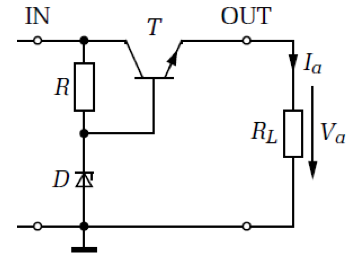
\includegraphics[width=6cm]{images/transistorStabilisierung}
		\end{minipage}
	&
		\begin{minipage}{8cm}
			\begin{gather*}
				U_{A}=U_{Z}-U_{BE}\\
				R_{V}=\frac{U_{E}-U_{Z}}{I_{Z}+I_{B}}\\
				I_{B}=\frac{I_{C}}{B}\\
				I_{C} \approx I_E = I_L \\
				R_{i}\approx\frac{r_{Z}}{\beta} 
			\end{gather*}
			
			\begin{tabular}{ll}
				$U_{Z}$:&Z-Dioden-Spannung\\
				$I_{Z}$:&Strom durch die Z-Diode\\
				$R_{i}$:&Innenwiderstand der Schaltung\\
				$r_{Z}$:&dyn. Innenwiderstand der Z-Diode\\
				$B$:&Gleichstromverstärkung \\
				$\beta$:&Dynamische Verstärkung \\
			\end{tabular}
		\end{minipage}
	\\ \hline
		\begin{minipage}{4cm}
			\textbf{Lineare Regler}
		\end{minipage}
	&
		\begin{minipage}{6cm}
			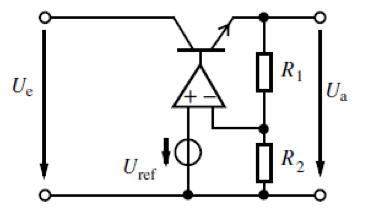
\includegraphics[width=6cm,trim=0 0 -5 -5]{images/linearRegler}
		\end{minipage}
	&
		\begin{minipage}{8cm}
			\begin{gather*}
				U_a = \left( 1+ \frac{R_1}{R_2} \right) \cdot U_{ref}
			\end{gather*}
			Erhältlich als integrierte Regler, z.B. 78xx \\
			Spannungsabfall $\approx 2V$ \\
			\\
			Low-Dropout-Regler (LDO): PMOS-FET anstatt Transistor \\
		\end{minipage}
	\\ \hline
		\begin{minipage}{4cm}
			\textbf{Lineare Regler mit einstellbarer Ausgangsspannung}
		\end{minipage}
	&
		\begin{minipage}{6cm}
			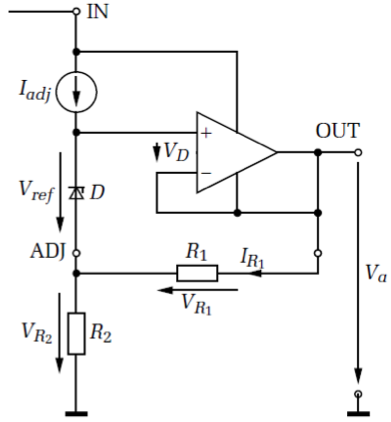
\includegraphics[width=6cm, trim=0 0 0 -5]{images/einstellbarStabilisierung}
		\end{minipage}
	&
		\begin{minipage}{8cm}
			Adjust-Pin (ADJ) zum Anschluss der externen Widerstände $R_1,R_2$
			\begin{gather*}
				U_a = U_{R_1} + U_{R_2} = U_{ref} + R_2 \cdot 
				\left(\frac{U_{ref}}{R_1} + I_{adj}\right) \\
				\text{für }I_{adj} \ll I_{R_1} \text{gilt:} \\
				U_a = U_{ref} \cdot \left(1+\frac{R_2}{R_1}\right)
			\end{gather*}
		\end{minipage}
	\\ \hline
\end{longtable}

\subsection{Schaltregler}
	\subsubsection{Grundprinzip}
		Energie wird in verlustarmem Element zwischengespeichert und auf gewünschter
		Spannung stabilisiert. Als Energiespeicher kommen in Frage: \textbf{Kondensatoren}
		für kleine Leistungen und \textbf{Spulen} für mittlere bis grosse Leistungen.
		Übliche Schaltfrequenzen liegen im Bereich von $200kHz$. \\
		
		Energie wird im Magnetfeld gespeichert: $E_L = \frac{L}{2} \cdot i_L^2$ \\
		Spannung über Spule bewirkt Stromänderung: $I_L = \frac{1}{L} \int V_L(t) \, dt$ \\
		Kondensator am Ausgang stabilisiert Spannung \\
		
		\begin{minipage}{8cm}
			\textbf{Abwärtswandler} (Step-Down, Buck Converter) \\
			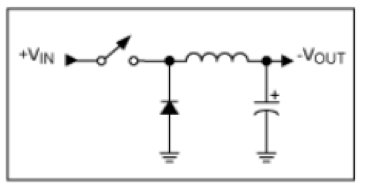
\includegraphics[width=6cm]{images/buckConv} \\
			\textbf{Invertierender Wandler} (Inverting) \\
			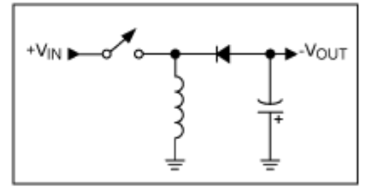
\includegraphics[width=6cm]{images/invConv} \\
		\end{minipage}
		\begin{minipage}{8cm}
			\textbf{Aufwärtswandler} (Step-Up, Boost Converter) \\
			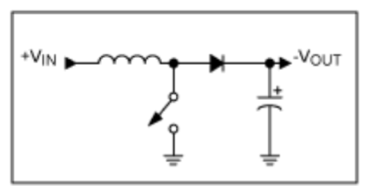
\includegraphics[width=6cm]{images/boostConv} \\
			\textbf{Sperrwandler} (Flyback Converter) \\
			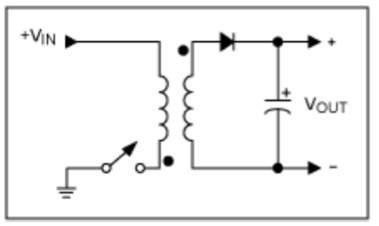
\includegraphics[width=6cm]{images/flybackConv}
		\end{minipage}

\subsection{Effizienzsteigerung}
	\subsubsection{MOSFET statt Diode}
		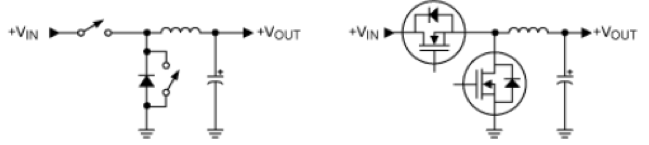
\includegraphics[width=12cm]{images/effizient1}
		\begin{itemize}
		\begin{minipage}{8cm}
 		 	\item Diode hat Spannungsabfall
  			\begin{itemize}
    			\item Silizium-Diode: 0.7V
   				\item Schottky-Diode: 0.3V
    			\item MOSFET hat "`nur"' On-Widerstand $R_{DS_{on}}$
			\end{itemize}
		\end{minipage}
		\begin{minipage}{8cm}
			\item Umschalten vom Substratpotential beim Längstransistor nötig
   			\begin{itemize}
     			\item Synchronous rectifier
    		\end{itemize}
		\end{minipage}
		\end{itemize}